\documentclass{acm_proc_article-sp}
\usepackage{url}
\begin{document}


%make title bold and 14 pt font (Latex default is non-bold, 16 pt)
\title{\Large \bf Social Math: A collaborative, visual host for mathematical proof trees}
\numberofauthors{4} %  in this sample file, there are a *total*
% of EIGHT authors. SIX appear on the 'first-page' (for formatting
% reasons) and the remaining two appear in the \additionalauthors section.
%
\author{
\alignauthor
Jianchi Chen\\
       \affaddr{Dept. of Electronical Engineering}\\
       \email{jchen2@caltech.edu}
\alignauthor
Ying-Yu Ho\\
       \affaddr{Dept. of Physics,}\\
       \affaddr{Mathematics, and Astronomy}\\
       \email{yingyu@caltech.edu}
\alignauthor
Tim Holland\\
       \affaddr{Dept. of Computing and}\\
       \affaddr{Mathematical Sciences}\\
       \email{th0114nd@gmail.com}
\and  % use '\and' if you need 'another row' of author names
\alignauthor 
Kexin Rong\\
       \affaddr{Dept. of Computing and}\\
      \affaddr{Mathematical Sciences}\\
      \email{krong@caltech.edu}
}

\maketitle

% Use the following at camera-ready time to suppress page numbers.
% Comment it out when you first submit the paper for review.
\thispagestyle{empty}

\subsection*{Abstract}
A mathematical proof has the structure of a DAG. However, it is typically
presented in a linear fashion, and cannot practically expose the depth of its
roots. We propose a web service to provide both of these by exposing part of
the graph to the user and allowing them to explore down into the subproofs.
Naturally it would be prohibitive for the authors to write even a useful amount
of the tree in, so the service allows the introduction of new proofs to expand
the reach of the proof trees. Specification of proofs could either be very
formal, in which case a program could verify them or more relaxed and reviewed
by other users in a social effort to find mathematical truth.

\section{Introduction}
We propose a web application that allows the inspection of, addition to, and
potentially input of verification of collection of large proof DAGs.
Interfacing with a node of the tree will present a statement of the theorem
associated with that node, edges to the children and potentially to some of its
parents. Text accompanies the node, and explains how the children are combined
together to prove the theorem. Ideally the accompanying text is as small as
possible and the nodes have a small fan out to break the proof down into
digestible chunks.

We have two possible choices to proceed on how to keep the DAG logically sound.
The first is more of a technical problem: require highly precise statements of
additions to the tree to be parsed, the logical statements can then be verified
(or rejected) automatically. Alternatively, with a more social emphasis proofs
could be stated in natural mathematical language. Under this scheme, the
correctness would have to be verified by users, through a combination
of moderation, reputation, and democracy.

\section{Technical Hurdles}
At the very basic level we have to deal with all the usual problems in
building a webapp: deciding upon tools (languages, databases, frameworks)
and an API to communicate between client and server. Further features
needed would be dynamic loading of the graph as the user scrolls through,
search to look for other proofs to minimize redundancy, automated theorem
verification or a voting mechanism, ability to mention other theorems
to include them is lemmas in a particular proof, text entry for a theorem,
inclusion of images for proofs that necessitate it, and collections of
axioms for the various fields of mathematics that could be present as
a starting point. Hard problems would involve the choice of data 
structure for the proofs, intuitive presentation of the DAG to the user,
an effective mechanism of rejecting poorly worded or incorrect proofs.

\section{Potential Order of Implementation}
\begin{enumerate}
    \item Persistent storage of a proof in the database.
    \item Communication of a proof over the network.
    \item User interface.
    \item Adding a new theorem from the user interface.
    \item Persistence of theorems in UI across page loads.
    \item Verification system (social or formal). 
\end{enumerate}

\section{Background}
I'm not aware of any similar projects.
% \bibliography{sample}}
% \theendnotes

\section{Timeline}
\subsection{Initial Timeline}
Below is the initial project timeline we proposed at the project proposal presentation. The plan was to build a working prototype before midterm, and to add as many features as time allows afterwards.  
\begin{itemize}
\item Week 2 - 5: Basics
\begin{itemize}
\item Client-server API
\item Database API
\item Implement views and templates for browsing, editing, and adding theorems
\item Front end visualization
\end{itemize}
\item Week 6: Milestone:\\
Should have a simple working prototype, which allows adding, deleting and viewing nodes from the proof DAG
\item Week 7 - 9: Useful advanced features
\begin{itemize}
\item Search by keywords
\item User profile
\item Private graph
\item Auto-keyword-extraction
\item Suggested theorems
\end{itemize}
\end{itemize}

\subsection{Actual Timeline}
Below is a summary of our actual weekly progress based on the blogs. The front end progress was highly non-linear because we either underestimated the amount of work or overestimated the ability to stick to schedule of the person in charge. Thus most features were first implemented on the server-side, and then enhanced with Ajax. Nevertheless, we were able to implement the three most useful advanced features: keyword search, user profile and private graph. A detail description of the end product is given in the next section.
\begin{enumerate}
\item \emph{Week 1: Changing Gears}\\\\
Due to the discovery of a fairly comprehensive open source traffic simulator project, we decided to abandon the original 144 project proposal and to work, instead, on a web application that accommodates the visualization of mathematical proof tree structures. We discussed the basic application architecture, and decided to use the typical LAMP stack with a REST API and CRUD functionality. In our case the P stands for Python with Django REST framework, the M stands for SQLite, and the A could either be Apache or Amazon Web Service.\\\\
The first steps we took were similar to any team making a CRUD app: setting up the database and a method of communication between the client and server. Specifically, we determined a schema for the database and fleshed out data structures for the DAG. We also started to familiarized ourselves with the frameworks that we will be working with for the rest of the term.\\\\
On the front end side, several JavaScript frameworks quickly came to our mind:
AngularJS\cite{Google:2014:Online} and/or jQuery for DOM manipulation, Bootstrap\cite{UI:2014:Online} for style and UI components, and D3.js \cite{Bostock:2014:Online} for data visualization. These frameworks have some overlapping functions so it was important to use them in a way that avoided conflicts and, preferably, reflected separation of concerns. Since we had  very little experience in web development, it took a significant amount of time to study JavaScript and its frameworks before we could make design decisions.\\\\

\item \emph{Week 2: Getting Started }\\\\
This week, the first draft of the API was written. It's a fairly
standard one that supports the collection of all entries in
a paginated manner, getting a single entry for a close up view,
and the CRUD operations. \\\\
On the server side, we've decided to go for AWS instead of Apache. As a result, we switched to using virtualenv, which gave us consistent versioning across our local machines, as well as allowing us to use versions required by AWS without having conflicts of the development computers. We also migrated from SQLite to MySQL, since AWS had the best support for the latter. Although setting up MySQL was slightly frustrating.\\\\
On the backend side, we implemented serializers to help form JSON responses, and view methods for creating and reading theorems/proofs.\\\\
On the front end side, we started by finding data visualization examples to understand the power of available tools. One of our particular interest was d3 process map \cite{Nylen:2014:Online}, which demonstrated a hierarchical layout of graph that we could potentially mimic. Meanwhile, we realized that AngularJS, jQuery, and D3.js all provided DOM manipulation methods. To avoid potential conflicts among the three frameworks,  we decided to structure front end applications on MVC (model-viewer-controller) framework of AngularJS, avoid jQuery as much as possible, and use D3.js mainly as a graph layout engine. No JavaScript codes were written yet, but we were able to write some Django view templates to provide text-based interaction with DAG.\\

\item \emph{Week 3: Backend Milestone}\\\\
After adding templates and view methods for editing and deleting, we had a fully working set of CRUD functionality implemented this week. We also did substantial unit tests on database models and api calls to make sure that our backend infrastructure had been robust so far. \\\\
At this point, the backend side has already reached the original midterm milestone. On the front end side, we succeeded in driving AngularJS templates with D3 graph layout engine. However, the hierarchical force layout algorithm in d3 process map wasn't as useful as we had expected. While D3.js provided nice force layout algorithm, it required users to manually specify the hierarchy relationships in the dataset.  Therefore, we started to design our own algorithm. Another obstacle was that we formatted graphs as adjacency lists while D3 Force Layout used nodes and edges as native objects. Therefore, proper conversion was needed in order to make use of the D3 framework.\\

\item \emph{Week 4: Frontend Milestone}\\\\
After reaching the milestone, the backend side has moved on to advanced features, starting with the keyword related ones. We first implemented functionalities for keyword creation, edit and search . Users can now tag theorems and proofs with appropriate  keywords.  A search bar was added on the index page to allow search by keywords.\\\\
As we moved one person from the backend to the front end, the front end side was able to make substantial progress this week. We wrote a stylesheet for the website to make it more user friendly. We also set up MathJax \cite{MathJax}, a free online LaTeX compiling tool, to support adding and displaying LaTeX code on the website. Finally, we built a client-side knowledge graph editor that made it possible to implement and test a working graph layout algorithm. This graph editor also served as an exercise on Bootstrap UI components and a reference of our final user interface. The next step was to turn the graph editor into an Ajax application that was able to communicate with the server.\\

\item \emph{Week 5:  Prototype online}\\\\
This week, we have been focusing on putting a simple working version of our product online. On one hand, we tried to connect the knowledge graph visualization with backend database. On the other hand, we worked on setting up Amazon EC2 (Amazon Elastic Compute Cloud) to host the website. We were able to seed the database with number theory theorems and deploy the latest backend code. Knowledge graph visualization was not fully integrated yet, due to bugs in API for Ajax calls. \\\\
Meanwhile, we have also been extending the website's functionalities. We started to implement user authentication system, in the hope of enabling users to set up private knowledge graphs for classroom settings in the future.\\


\item \emph{Week 6: Makeover}\\\\
We did a makeover to the website by refactoring the HTML files using UI Bootstrap. We also redesigned the index page so that it could nicely combine the graph visualization with the search functionality.  In addition, we finished implementing user authentication systems and user profile. This was our first step of incorporating the "social" component in the website. \\

\item \emph{Week 7:  Merging}\\\\
This week we successfully merged the backend Django framework with the front end graph editor for knowledge graph visualization. We made a single-page application that can load latest submissions and perform searches via Ajax calls. We were also able to display all nodes and their dependencies in database with the graph layout algorithm. Future work was needed to make the visualization more interactive. \\\\
We extended user profiles to include recent activities, so users can keep track of their latest contributions. We started to keep track of users who published and last modified each theorem/proof. We also added a "following" feature for theorems to make it easier for users to keep up with their interests.  We moved the website to a new domain: socmat.com/prooftree.\\


\item \emph{Week 8: MVP}\\\\
This week we further polished the product. For the front end, we merged and deployed user profile related features. We were able to add a few interactive features to the knowledge graph:
\begin{enumerate}
\item Zoom and Panning: Since it is hard to fit the entire knowledge graph on the index page, we decided, instead, to giver users full control of which part of the graph they would like to see. 
\item Recenter: In addition to the global knowledge graph, we also allow users to view a local graph centered around any chosen node. This feature comes in handy when a user wants to explore a specific theorem/proof. By default, only the chosen node and its immediate neighbors are displayed in the local graph. However, users can adjust the number of higher-order neighbors shown from the interface.
\item Add child: This feature allows one to add a new theorem/proof directly from the knowledge graph. This serves as a more intuitive way for users to make contributions. 
\item Preview: This feature allows users to view the content of a node without redirecting to the detail page.
\end{enumerate}

Finally, we finished implementing private graphs, which was mainly designed for a classroom setting use case. Users can choose to create their own knowledge graphs, which will not be displayed on the public global graph. CRUD functionality and keyword search were also implemented in the private graph. 

\end{enumerate}
\section{End Product}
The end product would hopefully be a useful web application that would
allow publishing of proofs in a graphical format subject to immediate review
of other users, and a repository for a large collection of proofs to be
seen in a graphical format upon request.
\subsection{UI and Visualization}
\subsection{Web Framework}
The server middleware is based on the Django web-framework. It provides a full set of functionalities for socialmath users to conveniently contribute to the mathematical knowledge library and to build their own graph:
\begin{itemize}

\item \emph{Nodes and Dependencies} \\
The most fundamental functionality in the socialmath web framework is the node-dependency system. In the framework, the nodes contain information about its theme, content, type, publication and modification dates. We used relationship structures to store node-node relationship, as well as node-to-other-object relationships. 
\begin{figure}[h!]
\centering
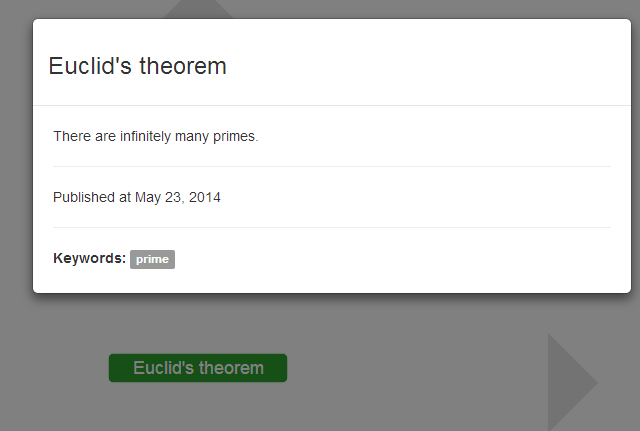
\includegraphics[scale=0.5]{oneNode.png}
\caption{One node in social math knowledge graph}
\end{figure}\\
Dependencies are classified into three types:
\begin{enumerate}
\item \emph{Proof-to-Theorem}: Lemma dependency. This relationship exists when a proof of one theorem cites another theorem in the proving process. 
\item \emph{Theorem-to-Proof}: Prove dependency. This relationship exists when a proof proves a theorem. 
\begin{figure}[h!]
\centering
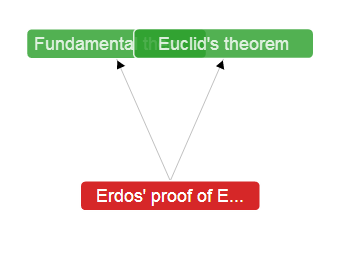
\includegraphics[scale=0.3]{prove_lemma_relationship.png}
\caption{Erdos' prove of Euclid's theorem exhibits prove relationship to Euclid's theorem, and exhibits lemma relationship to Fundamental Theorem of Arithmetic}
\end{figure}\
\item \emph{Theorem-to-Theorem}: High-Relevancy dependency. This relationship exists when a theorem is the special case or a broader case of another, or they have strong logical relationship with each other. This also includes the relationship between theorems and definitions, which we also model as theorems in our system (only that defs can't have proofs).
\begin{figure}[h!]
\centering
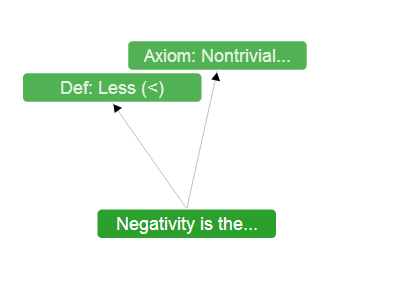
\includegraphics[scale=0.4]{tt_relationship.png}
\caption{Theorem-theorem and theorem-definition relationship}
\end{figure}\
\end{enumerate}

\item \emph{Keywords and Search} \\
Keywords are words that generalize a node's content and branch of study. They can be added upon adding the node, or can be added when editing an existing node. Node-keyword relationships are stored in a separate object named KWMap. 
\begin{figure}[h!]
\centering

\includegraphics[scale=0.8]{keyword.png}
\caption{Keywords in the detail-view of a node}
\end{figure}\\
The search functionality is supported by keyword mapping. Search can be used in two ways: you can either enter text in the search bar displayed at the index page, or you can click on the link of an existing keyword. 
\begin{figure}[h!]
\centering
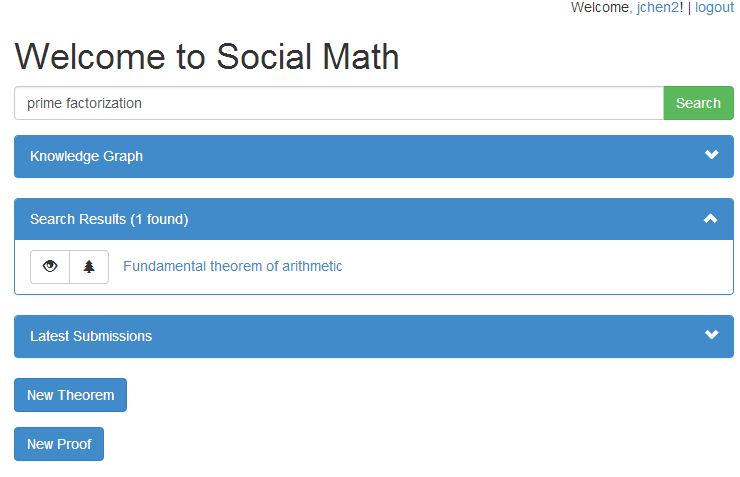
\includegraphics[scale=0.4]{search.png}
\caption{Search result for the keyword "prime factorization"}
\end{figure}\

\item \emph{Submission and Editing} \\
Adding a new theorem or proof can be done in two ways: 
Click on the button at the bottom of the index page, or use the "add child" tool on the graph. 
\begin{figure}[h!]
\centering
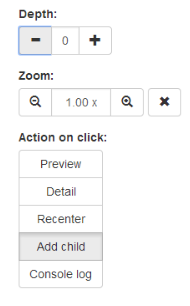
\includegraphics[scale=0.4]{add_child.png}
\caption{The "add child" tool}
\end{figure}\\
To edit an existing theorem, the user would have to go to the detail page and click on the "edit" button, where the user will see an interface similar to the add-node page, only that existing information has been filled in. 
\begin{figure}[h!]
\centering
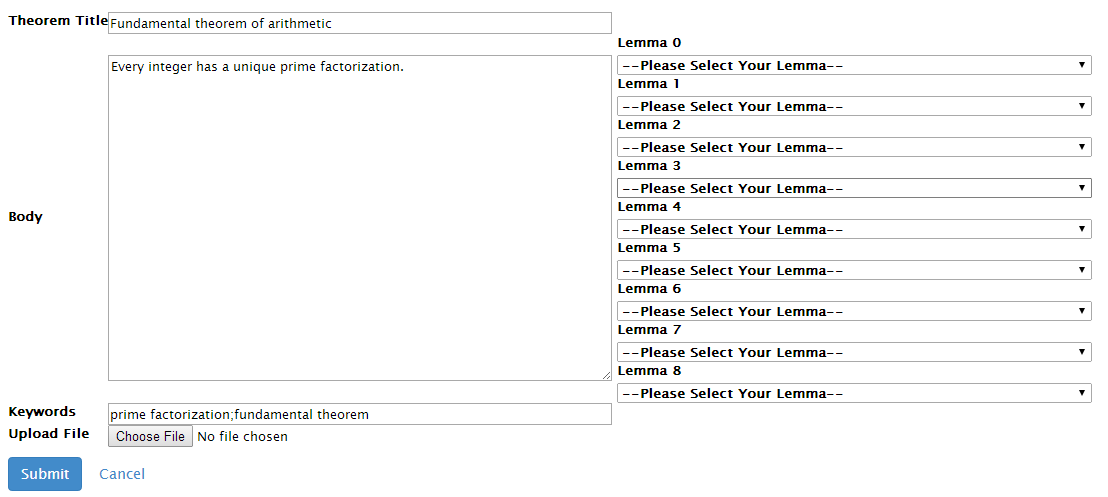
\includegraphics[scale=0.4]{edit.png}
\caption{Editing an existing node}
\end{figure}\\

\item \emph{Users and Profile} \\
Socialmath doesn't require a user to login to view its content, but there are additional functionalities for logged in users. 
\begin{figure}[h!]
\centering
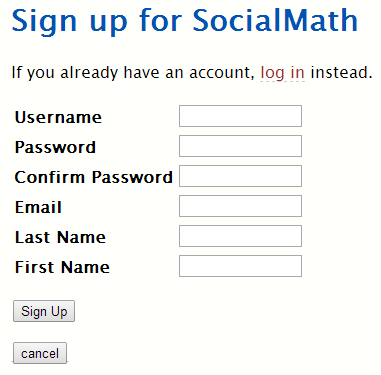
\includegraphics[scale=0.15]{signup.png}
\caption{User registration page}
\end{figure}\\
Once a user is logged in, every edition/addition activity will be recorded as an "event" in the database. They will show up both on the detail page of the node being edited, and on your own profile page as well. 
\begin{figure}[h!]
\centering
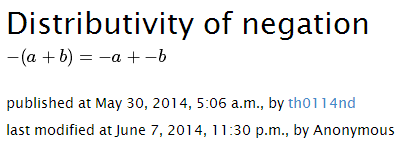
\includegraphics[scale=0.6]{edit_history.png}
\caption{Edition history of a node showing the initial author and the last modifier}
\end{figure}\\
\emph{Follow} is a functionality provided for registered users. The user may click on the "follow" button of any given node, and the server will record it as an event of "follow" type. 
To view a user's own profile, the user can always click on his own username on the top navigation bar. Right now, there is now search-for-user functionality, so the only entrance for viewing other users' profiles is in the edition history of nodes. 
\begin{figure}[h!]
\centering
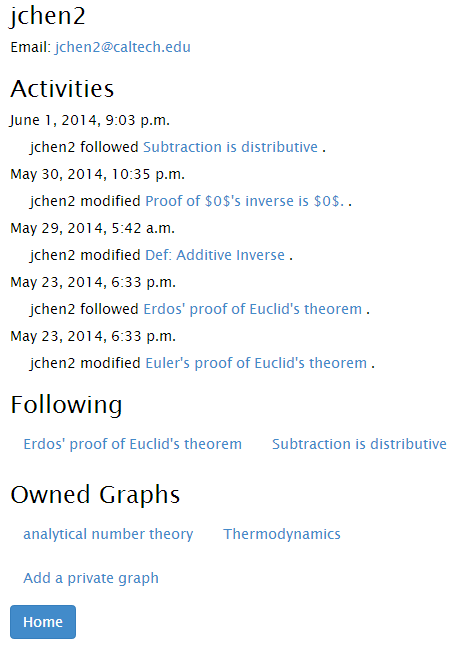
\includegraphics[scale=0.52]{profile.png}
\caption{The profile page of Jianchi Chen, consist of basic info, activities, following-nodes, and private graphs he owns}
\end{figure}\\

\item \emph{Private Graphs} \\
In addition to one public graph visible to everyone, socialmath also implemented a functionality called \emph{private graph} so that each registered user can create and edit his own graph. Upon creation, the user may choose to make the graph public or only disclosed to authorized users. 
\begin{figure}[h!]
\centering
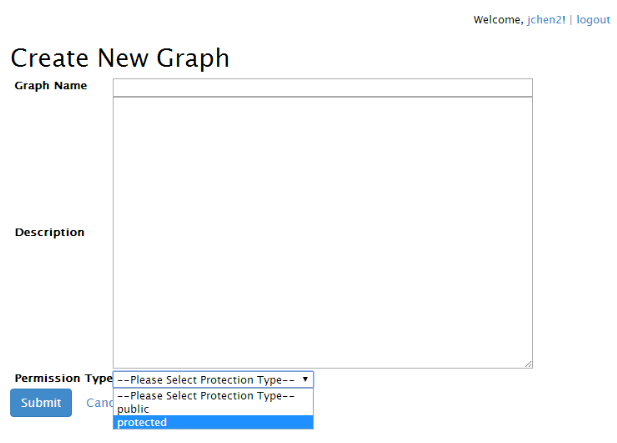
\includegraphics[scale=0.4]{create_pg.png}
\caption{Creating a private graph}
\end{figure}\\
The created private graph will have a individual index page, and every node added to the private graph will not show up on the public graph.  
\begin{figure}[h!]
\centering
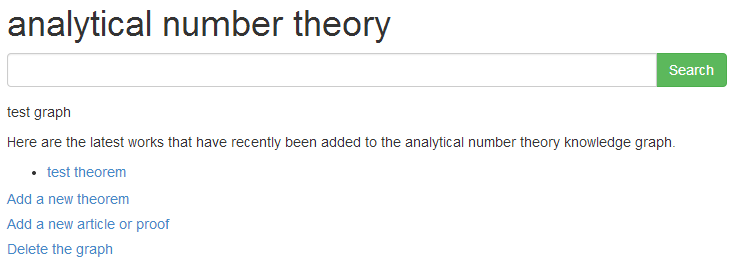
\includegraphics[scale=0.4]{pg_index.png}
\caption{The index page of a private graph, with a node called "test theorem" added.}
\end{figure}\\
All contents associated with a private graph will be visible to the owner and invited user only. An attempt to view private graph contents when you're not invited will result in a 401 unauthorized error. 

\end{itemize}

\subsection{Database}
\subsubsection{Entity-set Schema}
\begin{itemize}
\item Node(\underline{node\_id}, kind, title, statement, pub\_time, last\_modified)
\item Keyword(\underline{kw\_id}, word)
\item PrivateGraph(\underline{pgraph\_id}, name, description, pub\_time, perm\_type)
\item We used the default Django model for user authentication:
User(\underline{user\_id}, username, email, password, ...)\\ 
\end{itemize}

\subsubsection{Relationship-set Schema}
\begin{itemize}
\item Depend(\underline{node\_id}, \underline{node\_id}, dep\_type)
\item Tag(\underline{node\_id}, \underline{kw\_id})
\item Modify(\underline{node\_id}, \underline{user\_id}, pub\_time, event\_type)
\item Own(\underline{user\_id}, \underline{pgraph\_id})
\item Include(\underline{pgraph\_id}, \underline{node\_id})
\end{itemize}

\begin{figure}
\centering
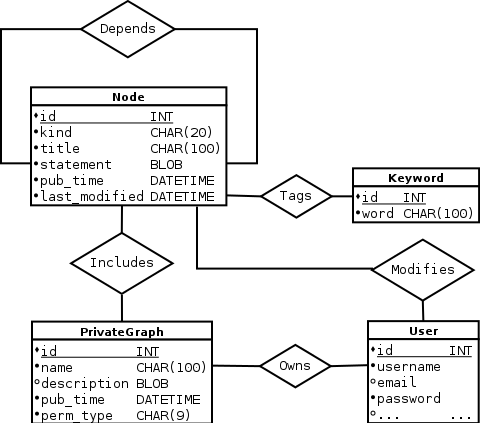
\includegraphics[scale=0.5]{socialmath_ER.png}
\caption{ER Diagram}
\end{figure}


\section{Future plans} 
Although we think that the current socialmath is ready for public usage, there are several additional goals that we plan to achieve with socialmath in the future in order to make it a better product:
\begin{enumerate}
\item \emph{Protection against malicious activity} \\
Right now, socialmath has no protection against a user who simply wants to delete everything on the knowledge graph, or change everything to spam. We plan to learn from how wikipedia prevents users from malicious editions, by having a more comprehensive edition history and revert-edition functionality, as well as user-penalty system. 
\item \emph{Correctness system} \\
Also, the website currently has no way of detecting correctness of a proof or a theorem. Multiple alternatives can be used in this regard: an user upvote system, or a user "questioning" system where users can request verification on statements, etc. 
\item \emph{A more complete private graph system} \\
An ideal model for a private graph will be a github repository, where users can collaborate and utilize multiple edition tools. Also, we will work to implement full visualization of the private graph so that it is the same as the global graph. 
\item \emph{File uploading} \\
Right now, socialmath only supports in-box writing. Although LaTeX formulas are supported, it would be more desirable if we can add pdf-uploading and displaying functionality. 
\item \emph{Lemma and keyword detection} \\
A more advanced version of the socialmath node submission system plans to have lemma and keyword auto-detection, where the system scans for heuristics in the content. 
\item \emph{Better user interaction system} \\
We plan to enhance the "social" side of socialmath. Search-for-user, follow-user, invite/messaging systems are all planned. 
\end{enumerate}

%ACKNOWLEDGMENTS are optional
\section{Acknowledgments}


%
% The following two commands are all you need in the
% initial runs of your .tex file to
% produce the bibliography for the citations in your paper.
\bibliographystyle{plain}
\bibliography{socialmath} 
% You must have a proper ".bib" file
%  and remember to run:
% latex bibtex latex latex
% to resolve all references
%
% ACM needs 'a single self-contained file'!
%
%APPENDICES are optional
%\balancecolumns

% That's all folks!

\end{document}
